
\section{Evaluation}
\label{sec:ev}

In this section, we analyze the performance of the \pnum~protocols that we have implemented over \odlib.
We start the discussion by providing a high-level overview of the 
key insights of this evaluation.
Then we individually analyze the performance of each class of protocols. 

\subsection{Overview} 
\label{sec:ev:ov}

\begin{figure*}[t]
\centering
  \begin{subfigure}[b]{0.33\textwidth}
    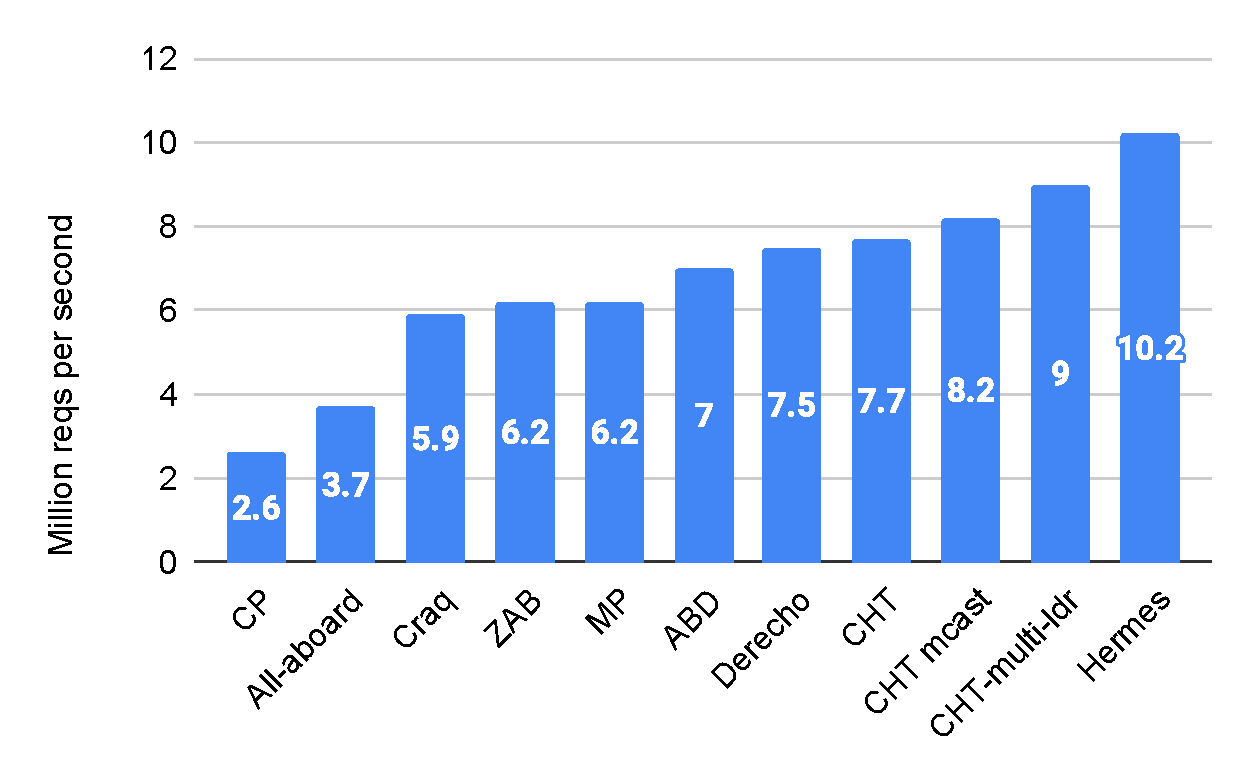
\includegraphics[width=\textwidth]{1_figures/single-thread.pdf}
    % \captionsetup{width=0.85\linewidth}
    % \vspace{-1.8em}
    \caption{Single-threaded write throughput}
%   \vspace{-1.5em}
  \label{fig:single-thr}
  \end{subfigure}
  %
  \begin{subfigure}[b]{0.33\textwidth}
    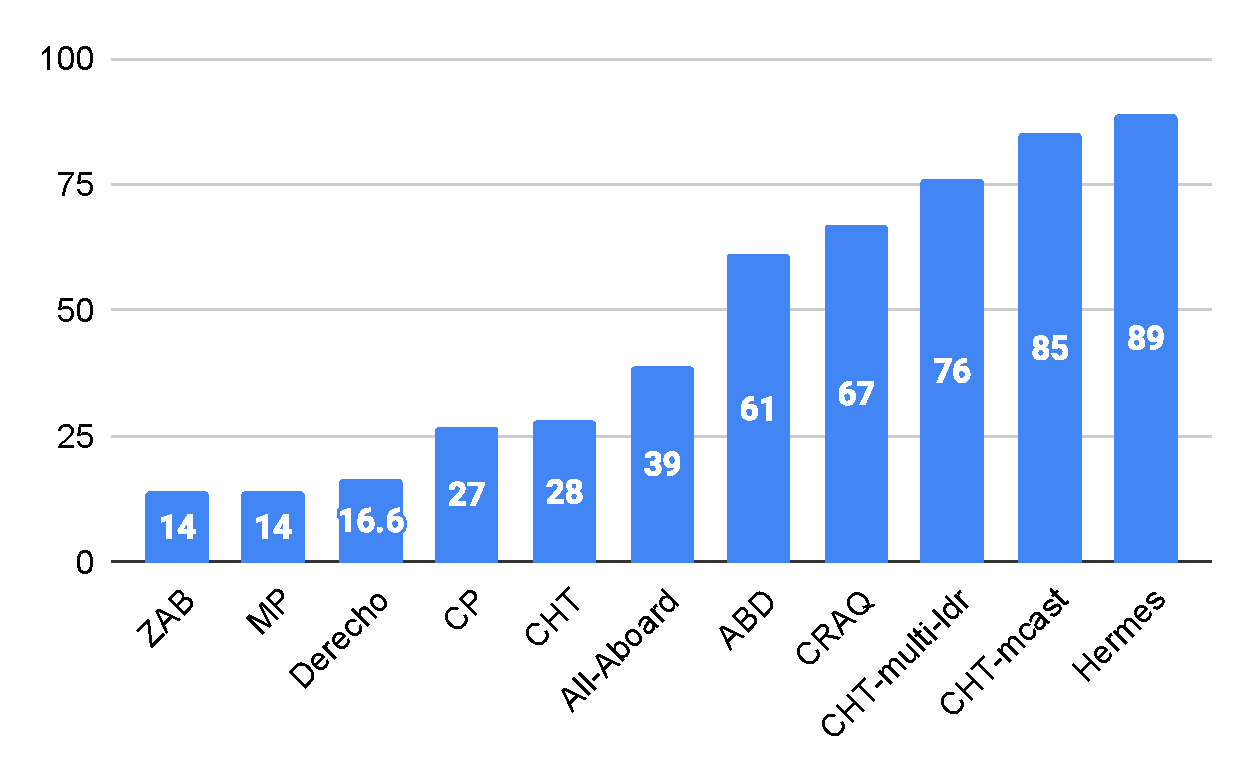
\includegraphics[width=\textwidth]{1_figures/Write-only-chart.pdf}
    % \captionsetup{width=0.85\linewidth}
    % \vspace{-1.8em}
    \caption{Multi-threaded write throughput}
    %   \vspace{-1.5em}
  \label{fig:write-all}
  \end{subfigure}
  %
  \begin{subfigure}[b]{0.33\textwidth} 
  
    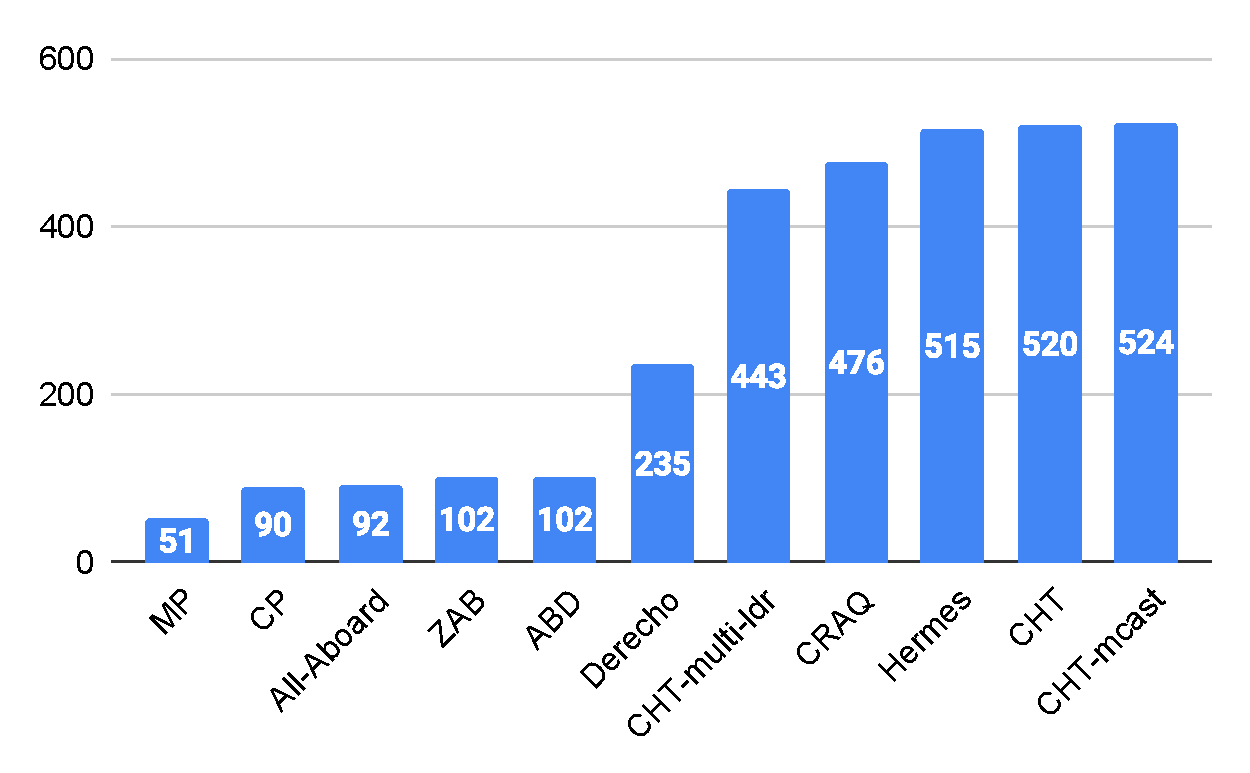
\includegraphics[width=\textwidth]{1_figures/5perc-writes.pdf}
    % \captionsetup{width=0.85\linewidth}
    % \vspace{-1.8em}
    \caption{Multi-threaded throughput at 95\% reads}
%   \vspace{-1.5em}
  \label{fig:5perc}
  \end{subfigure}
%   \vspace{-1em}
  \caption{Throughput comparison of all protocols in M.reqs/s. Note that both the x-axes and y-axes are different in each graph.}
 %\antonis{caption is closer to the text below than the subcaptions above}}
  \label{fig:three-bars}
%   \vspace{-1em}
\end{figure*}

First, we briefly describe \figref{fig:three-bars} and \tabref{tab:all-perf} and then analyze our key insights and provide general directives and recommendations. 

\beginbsec{\figref{fig:three-bars}}
\figref{fig:three-bars} shows the throughput of all protocols in million requests per second (M.reqs/s), ordering the protocols in ascending throughput order. 
Specifically, \figref{fig:single-thr} and \ref{fig:write-all} show the write throughput of the protocols when they are single-threaded and multi-threaded (default scenario), respectively.
Finally, \figref{fig:5perc} shows the throughput (multi-threaded), with 95\% reads.




Note the following three remarks for \figref{fig:three-bars}.
Firstly, both the x-axis and y-axis are different in all three graphs. Crucially, protocols in the x-axis are ordered in ascending throughput order.
Secondly, MP and ZAB are the same protocol in the write-only workload, \ie in \figref{fig:single-thr} and \ref{fig:write-all}, because they only differ in the execution of reads.
Third and final, note that there is a protocol called \emph{CHT-mcast}: this is the CHT protocol with the hardware multicast enabled. We show its performance separately because it performs significantly better than CHT. Enabling the multicast in the rest of the protocols has a very small impact. %

\beginbsec{\tabref{tab:all-perf}}
The left-hand side of \tabref{tab:all-perf} shows the throughput in M.reqs/s of all protocols when varying the write ratio. 
The right-hand side shows the latency (99th / average) of all protocols in microseconds at 100\% write ratio, while varying the load of the protocol (\ie with respect to peak throughput). 

\custvspace
\noindent
Let us now summarize the key insights from this study.


\beginbsec{1. Total order is not thread-scalable}
Protocols that apply writes in a total order are not thread-scalable:
the relative positions of ZAB, MP (\LTO), and Derecho (\DTO) in \figref{fig:single-thr} and \figref{fig:write-all} demonstrate this point. The reason is that explicitly enforcing total order mandates that threads can only apply writes to the KVS in lock-step.
In contrast, protocols that enforce per-key order (\LPKO~and \DPKO) can scale well with more threads.

\beginbsec{2. The leader jeopardizes load balance}
The adverse effect of the leader on load balance is not apparent in \LTO~protocols because they cannot scale enough to uncover it.
However it is visible in \LPKO~protocols.
Specifically, CHT does not scale well when multi-threaded because the send side of the leader becomes the bottleneck. %
There are two protocol-level optimizations that restore load balance: propagating writes through a chain (\ie CRAQ) and using multiple leaders (\ie CHT-multi-ldr).

\beginbsec{3. Hardware multicast is effective for \LPKO}
The hardware multicast primitive can make a huge difference, but only in \LPKO~protocols.
Specifically, the hardware multicast primitive provides a 3x benefit for CHT, i.e., CHT-mcast. 
The benefit for the rest of the protocols is very small, typically around 5\%.
The reason is that the multicast only relieves load on the send side of the node that performs the broadcast: it reduces the number of messages sent, but not the number of messages received.
Therefore, multicast is extremely useful for leader-based protocols that are bottlenecked by the send bandwidth of the leader. It is not so useful for already well-balanced protocols (\ie \DTO\  and \DPKO), while \LTO\ protocols do not benefit, as they are already bottlenecked by thread-scalability. We will expand in \secref{sec:ev:lpko}.%

\beginbsec{4. \DPKO~excels when multi-threaded}
In the absence of a leader or a total order, \DPKO\ protocols must find creative ways to serialize writes in a decentralized manner.
On the one hand, this invites a level of complexity that has an adverse affect on the work-per-request ratio. 
This is portrayed by the single-threaded performance of CP and All-Aboard, which is the lowest among all protocols.
On the other hand, the decentralized nature of these protocols makes them
naturally thread-scalable and load balanced. This is why multi-threading yields a $\sim$9-10x throughput improvement.
Notably, by downgrading the availability guarantees, as in Hermes, or downgrading the API, as in ABD, it is possible reduce the work-per-request ratio.

\beginbsec{5. Thread-scalability > load balance > work-per-request}
From \figref{fig:write-all}, we observe that the non-thread-scalable protocols, ZAB, MP and Derecho are the worst performers, rendering thread-scalability the most critical property to honour in the modern era.
Furthermore, All-Aboard, a protocol with a very high work-per-request ratio, significantly outperforms CHT, which sacrifices load balance, even though CHT offers lower availability guarantees (discussed in \S\ref{sec:fail}).
From that we concur that it is preferable to optimize for load balance rather than work-per-request ratio. At the limits of the work-per-request ratio (\ie in CP), the two metrics appear equally important, as CHT and CP are roughly matched.




\beginbsec{6. Local reads are great but with caveats}
Recall that MP performs reads by sending them to the leader. CP, All-aboard and ABD perform ABD-reads (typically 1 broadcast round). The rest perform reads locally.
From \figref{fig:5perc}, we see that there is a big gap between protocols with local reads and the rest, which perform them remotely. However there are a couple of caveats.
Firstly, local reads always come at a cost as they downgrade either the consistency or the availability guarantees, as we saw in \secref{sec:fail}.
Furthermore, note that ZAB, even though it performs its reads locally, is on par with the protocols that perform reads remotely.
This is because it is bottlenecked by its write throughput.
We elaborate in \secref{sec:ev:lto}.


\beginbsec{7. For better latency, choose throughput}
In the Introduction, we hypothesized that a request's latency should not exceed a few tens of microseconds in a lightly loaded system. 
Furthermore, we argued that to ensure a low latency, we should favour high-throughput protocols. %
The latency measurements for 25\% load in \tabref{tab:all-perf} verify that at a light load, all protocols incur a latency of a few tens of microseconds. 
Furthermore, we observe that for all protocols, as load increases so does latency, with a big spike at 100\% load. Therefore, to maintain a latency of a few tens of microseconds, 
one should favour high-throughput protocols, as they will be less likely to be overloaded when operating on the target throughput. %





\beginbsec{Summary -- Recommendations}
Based on our insights, we first provide some general directives on protocol design and then offer recommendations on choosing a protocol.

\beginbsec{General Directives}
\squishlist
\item %
Prioritize thread-scalability, then load-balance and then the work-per-request ratio.
\item Total order should be avoided in read/write systems.
\item Leader-based protocols can achieve high-performance, but care must be taken to ensure load balance. 
\item It is worth investing in the hardware multicast primitive only in the case of \LPKO\ protocols. 
\item Local reads can deliver great performance, but it's not guaranteed.
\item In order to minimize latency, choose protocols with high throughput.
\squishend
\noindent\textbf{Recommendations}
\squishlistContrib
\item All-aboard is the most attractive design point for a scenario where: 1) availability is the most important concern and 2) conditional writes are required.
\item If simple writes will do, then we recommend ABD.
\item If a small window of unavailability on a failure is tolerable, then Hermes is the best candidate, while CHT-multi-ldr and CRAQ are good alternatives.
\squishend 




\begin{figure*}[t]
\centering
  \begin{subfigure}[b]{0.33\textwidth}
    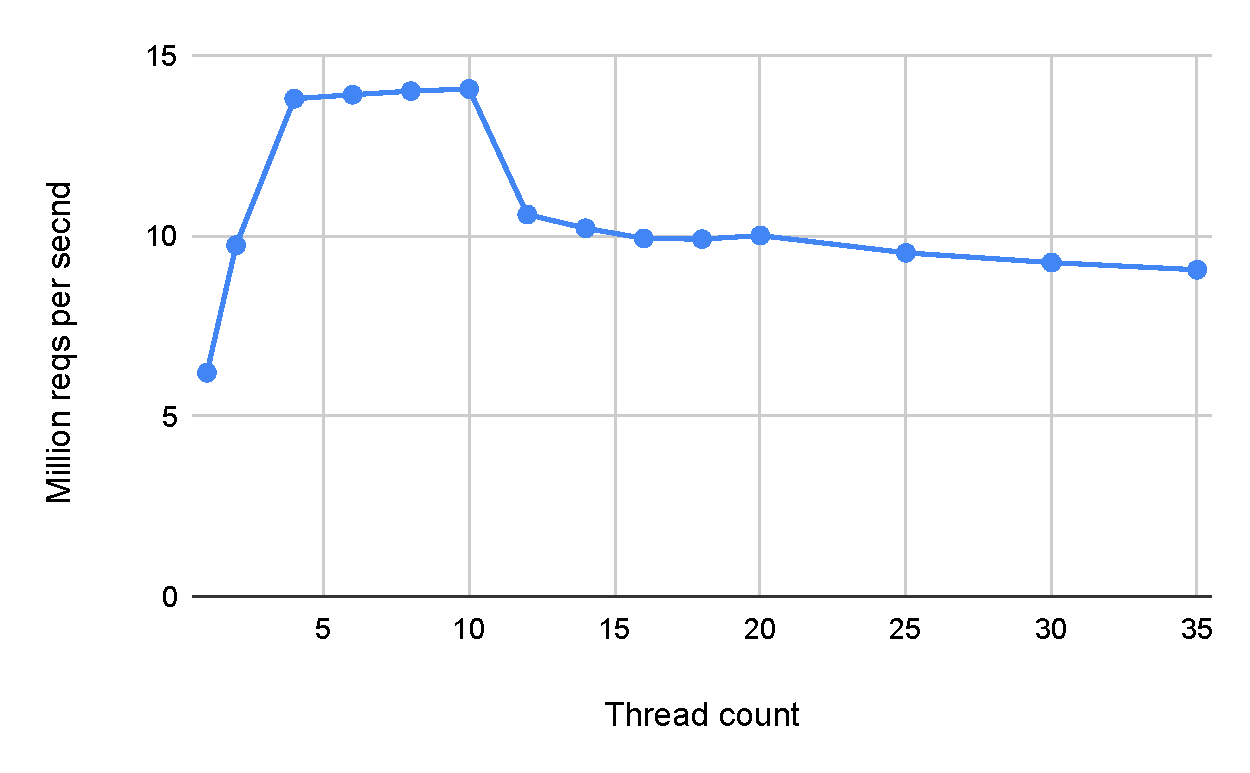
\includegraphics[width=\textwidth]{1_figures/ZAB-scal.pdf}
    \captionsetup{width=0.85\linewidth}
    % \vspace{-1.8em}
    \caption{Write-only throughput vs. thread cound for ZAB and MP}
%   \vspace{-1.5em}
  \label{fig:zab-scal}
  \end{subfigure}
  %
  \begin{subfigure}[b]{0.33\textwidth}
    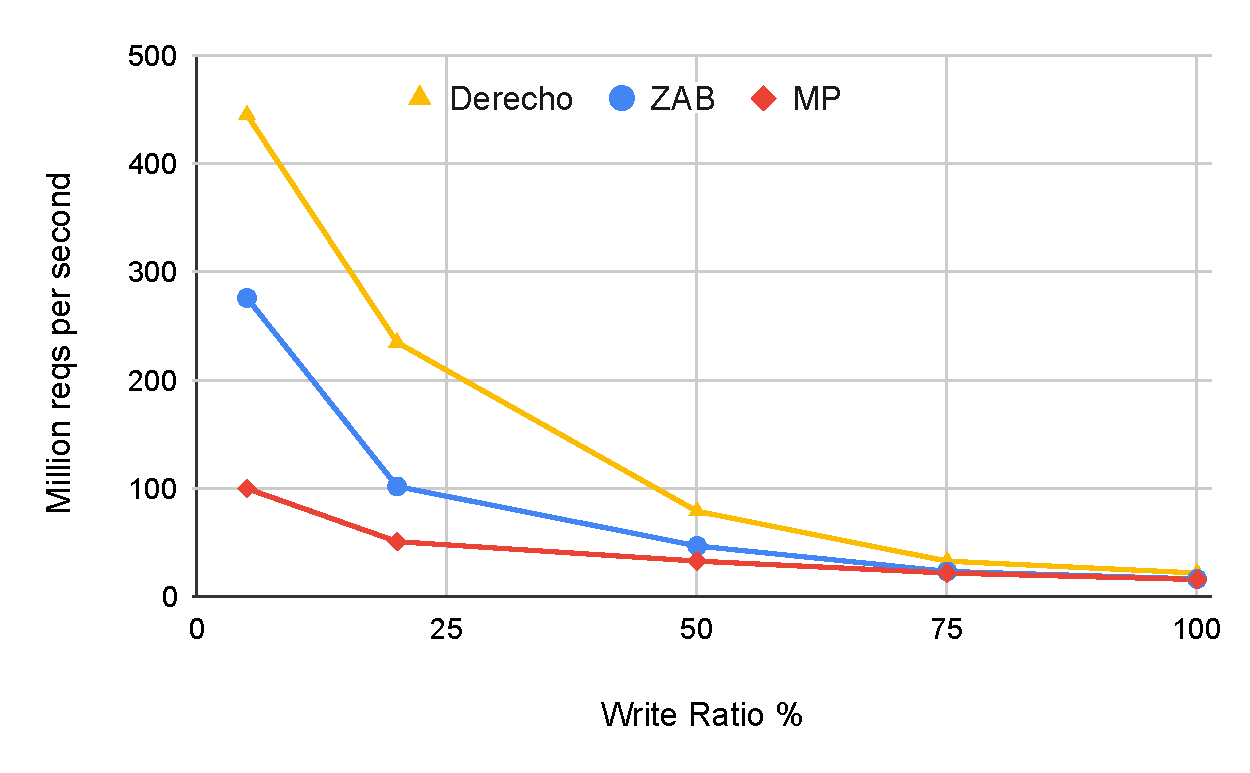
\includegraphics[width=\textwidth]{1_figures/zab-mp-dr.pdf}
    \captionsetup{width=0.85\linewidth}
    % \vspace{-1.8em}
    \caption{Throughput vs. write ratio for ZAB, MP \& Derecho}
    % \vspace{-1.5em}
  \label{fig:zab-mp-dr}
  \end{subfigure}
  %
  \begin{subfigure}[b]{0.33\textwidth} 
  
    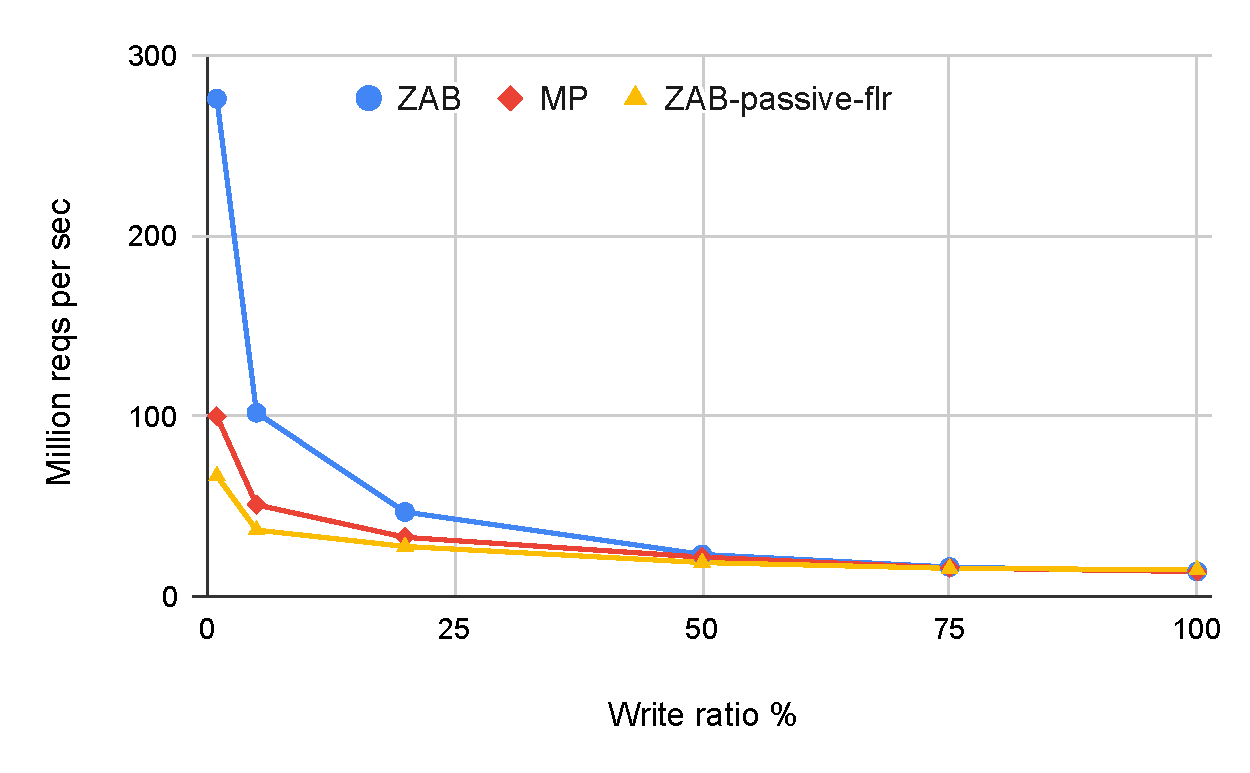
\includegraphics[width=\textwidth]{1_figures/zab-passive-flr.pdf}
    % \captionsetup{width=0.85\linewidth}
    \vspace{-1.8em}
    \caption{Throughput vs. write ratio for ZAB, MP and ZAB/MP with passive followers}
%   \vspace{-1.5em}
  \label{fig:zab-psv}
  \end{subfigure}
%   \vspace{-1em}
  \caption{Comparing ZAB, MP \& Derecho}
  \label{fig:lto}
%   \vspace{-1em}
\end{figure*}


% \begin{figure*}[t]
% \centering

% \begin{subfigure}[b]{0.33\textwidth}
%     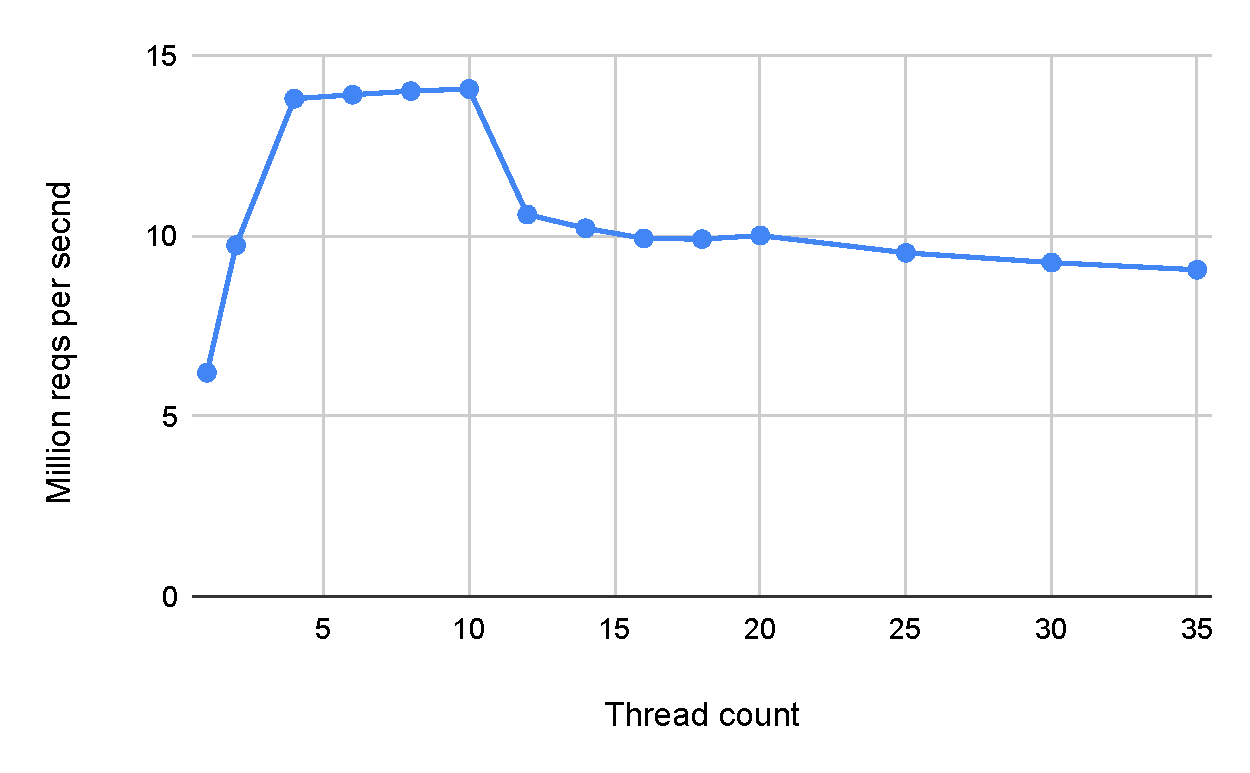
\includegraphics[width=\textwidth]{1_figures/ZAB-scal.pdf}
%     % \captionsetup{width=0.85\linewidth}
%     % \vspace{-1.8em}
%   \caption{Write-only throughput of ZAB and MP, varying the workers}
% %   \vspace{-1.5em}
%   \label{fig:zab-scal}
%   \end{subfigure} %%
  
% \begin{subfigure}[b]{0.33\textwidth}
% 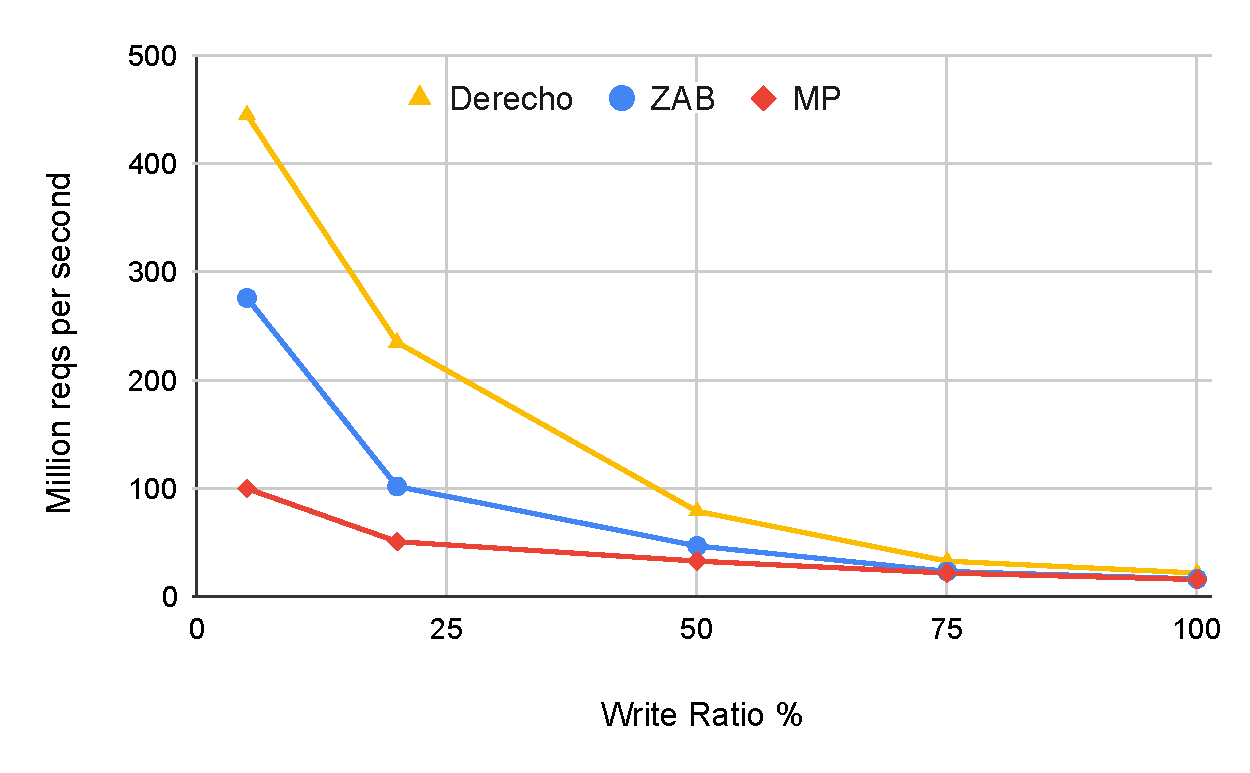
\includegraphics[width=\textwidth]{1_figures/zab-mp-dr.pdf}
% % \captionsetup{width=0.85\linewidth}
% % \vspace{-1.8em}
% \caption{Throughput of ZAB, MP \& Derecho, varying the write ratio from 1\% to 100\%}
% %   \vspace{-1.5em}
% \label{fig:zab-mp-dr}
% \end{subfigure}%

% \begin{subfigure}[b]{0.33\textwidth} 

% 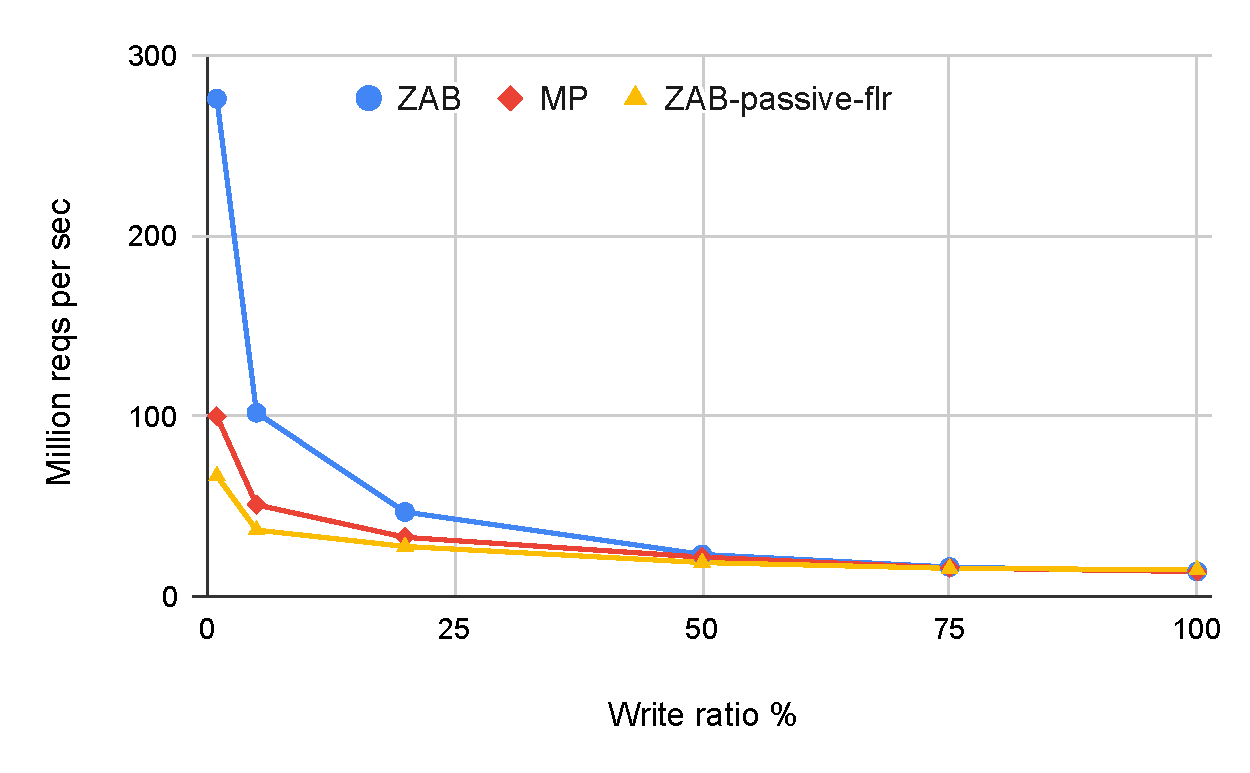
\includegraphics[width=\textwidth]{1_figures/zab-passive-flr.pdf}
% %   \vspace{-0.5em}
% \caption{Throughput of ZAB, MP and ZAB/MP with passive followers, when varying the write ratio}
% %   \vspace{-1.5em}
% \label{fig:zab-psv}
% \end{subfigure}%
% %   \vspace{-2em}
% \caption{\LTO~graphs. }
% \label{fig:lto}
% %   \vspace{-1.5em}
% \end{figure*}
\begin{table}[t]
\centering
 \resizebox{0.48\textwidth}{!}{%
\begin{tabular}{c|c|c|c|c|c|c|c|||c|c|c|c|c|}
\hhline{~-----------}
& \multicolumn{7}{c|||}{\colorhl\textbf{ Throughput vs. Write ratio}} &
\multicolumn{4}{c|}{\colorhl\textbf{ Latency vs. Load}}
 \\ 
 \hhline{~-----------}


\textbf{}                                                               
& 
 \colorhl%
{0\%} &
 \colorhl%
{1\%} &
 \colorhl%
{5\%} &
 \colorhl%
{20\%}&
 \colorhl%
{50\%}&
 \colorhl%
{75\%}&
 \colorhl%
{100\%} & 

 \colorhl%
{25\%} &
 \colorhl%
{50\%} &
 \colorhl%
{75\%} &
 \colorhl%
{100\%}
\\  
\hhline{~-----------}
\hline




\multicolumn{1}{|c|}{\colorhl ZAB} &
967 &	276 &	102 &	47 &	23.5 &	16.5 &	14 
& 
22 / 16 & 
30 / 23 & 
40 / 32 & 
110 / 95
 \\ \hline \hline
 \greyrow
\multicolumn{1}{|c|}{\colorhl MP} &
170 &	100 &	51 &	33 &	22 &	16 &	14 
&
22 / 16 & 
30 / 23 & 
40 / 32 & 
110 / 95
 \\ \hline \hline
\multicolumn{1}{|c|}{\colorhl Derecho} &
967 &	445 &	235 &	79 &	33 &	22 &	16.6 
&
16 / 13 & 
24 / 19 & 
32 / 27 & 
94 / 86
 \\ \hline \hline
 \greyrow
  \multicolumn{1}{|c|}{\colorhl CP} &
125 &	115 &	90 &	65 &	44 &	35 &	27 
&
38 / 26 & 
40 / 33 & 
56 / 47 & 
216 / 163
 \\ \hline \hline
\multicolumn{1}{|c|}{\colorhl CHT} &
967 &	755 &	520 &	134 &	53 &	36 &	28 
&16 / 16 & 
24 / 19 & 
38 / 31 & 
282 / 209
 \\ \hline \hline
 \greyrow
\multicolumn{1}{|c|}{\colorhl All-Aboard} &
125 &	116 &	92 &	70 &	51 &	42 &	39 
&
24 / 18 & 
38 / 27 & 
58 / 40 & 
252 / 167
 \\ \hline \hline
\multicolumn{1}{|c|}{\colorhl ABD} &
125 &	118 &	102 &	84 &	71 &	64 &	61 
&
28 / 26 & 
34 / 33 & 
52 / 47 & 
138 / 163
 \\ \hline \hline
 \greyrow
 \multicolumn{1}{|c|}{\colorhl CRAQ} &
967 &	739 &	476 &	246 &	123 &	87 &	67 
&
34 / 22 & 
48 / 30 & 
58 / 37 & 
242 / 138
 \\ \hline \hline
\multicolumn{1}{|c|}{\colorhl CHT-multi-ldr} &
967 &	674 &	443 &	192 &	134 &	97 &	76
&30 / 19 & 
82 / 58 & 
86 / 59 & 
554 / 323

 \\ \hline \hline
 \greyrow
\multicolumn{1}{|c|}{\colorhl CHT-mcast} &
967 &	745 &	524 &	277 &	145 &	105 &	85 
&
20 / 14 & 
24 / 16 & 
40 / 26 & 
210 / 147
 \\ \hline \hline

\multicolumn{1}{|c|}{\colorhl Hermes} &
967 &	735 &	515 &	275 &	150 &	107 &	89 
& 18 / 13 & 
24 / 15 & 
36 / 22 & 
110 / 78 
 \\ \hline 


\end{tabular}%
 }
\caption{Left-hand side: Throughput in M.reqs/s varying the write ratio. Right-hand side: 99th percentile and average latency (99th/ avg) in $\mu$seconds varying the load in a write-only workload.}
\vspace{-1.5em}
\label{tab:all-perf}
\end{table}


















\subsection{\LTO: ZAB and Multi-Paxos}\label{sec:ev:lto}


In this section, we first briefly describe the operation of our two implemented \LTO~protocols: ZAB and Multi-Paxos (MP). 
Then we focus on their results, first discussing thread-scalability for write throughput, and then the throughput when varying the write ratio.



\beginbsec{ZAB \& MP operation}
All writes must be propagated to the leader which executes them in two broadcast rounds: a prepare round and a commit round.
The difference between ZAB and MP is in reads. ZAB executes reads locally downgrading consistency guarantees to SC.
MP offers lin, and so, all reads are sent to the leader.





\beginbsec{Thread-scalability}
The thread-scalability problem occurs when the different workers, either in the leader or the followers, try to apply the writes to the KVS. For example, the write with write-id = 200 (\ie write-200), can only be applied \emph{after} write-199 has been applied. If worker-0 is responsible for applying write-200, but not write-199, then 
worker-0 must wait until the worker responsible for write-199 applies it.
Therefore the thread-scalability problem rises from the fact that workers can only apply their writes to the KVS in lock-step. \figref{fig:zab-scal} shows the write-only throughput of ZAB and MP when varying the number of threads (\ie workers). 
Scaling saturates at four workers.
When deployed with more than 10 workers, the performance drops because the additional workers are pinned to the second socket of the server, hindering inter-thread communication.




\beginbsec{Throughput when varying the write ratio}
\figref{fig:zab-mp-dr} compares the throughput of ZAB and MP with Derecho, when varying the write ratio.
ZAB's consistency relaxation that allows for local reads pays off, as ZAB significantly outperforms MP in low write ratios. 

However, note that ZAB's write throughput does not scale well in low write ratios. For instance, at 5\% write ratio, ZAB achieves 102 M.reqs/s, which means that its write throughput is roughly 5 million per sec. Ideally, since local reads are fairly cheap, one might expect that ZAB should have been able to maintain its peak write throughput (14m at 100\% write ratio) at lower write ratios. Note that Derecho maintains its 16.6m write throughput at both 75\% write ratio and 50\% write ratio. Derecho is able to sustain its write throughput better due to its decentralized nature and thus outperforms ZAB in lower write ratios. In contrast, in ZAB (and MP), followers must send their writes to the leader which coordinates their execution. When decreasing the write ratio, the ability to batch multiple writes together into network packets and steer them into the leader is disrupted by the execution of reads, and so the write throughput cannot be maintained.



\beginbsec{Passive followers}
In order to examine whether it would be beneficial to spawn requests only at the leader node, \figref{fig:zab-psv} shows the throughput of \emph{ZAB-passive-flr}, a ZAB variant where followers are passive: \ie followers are not connected with clients and thus do not initiate the execution of requests. Rather, only the leader initiates requests, while followers are only used to help coordinate writes. 
In this case, MP and ZAB are identical, because in both protocols reads at the leader can execute locally.
ZAB-passive-flr can achieve the same write throughput as ZAB at 100\% write ratio because all writes must execute at the leader anyway. However, its performance degrades as reads increase. The reason is that the single node (\ie the leader) cannot compete with a 5-node deployment when it comes to executing local reads. Specifically, followers' cpu and memory resources must be utilized to scale at low write ratios. Therefore active followers that are responsible for client sessions are beneficial. This result holds for \LPKO~protocols, too.





\subsection{\DTO: Derecho}\label{sec:ev:dto}
We have already established the effects of the total order in write throughput and contrasted Derecho with ZAB and MP. 
Here we will briefly describe Derecho's operation and comment on its performance in lower write ratios, contrasting it with two \DPKO~protocols.



\beginbsec{Derecho operation}
In Derecho, writes are totally ordered and applied in that order. The different write-ids are statically pre-allocated to different nodes. Node-0 will propose writes $0$ to $N-1$, node-1 will propose writes $N$ to $2N - 1$, and so on.
Furthermore, Derecho performs reads locally, relaxing the consistency guarantees from lin to SC (similarly to ZAB). 


\beginbsec{Performance}
Without considering thread-scalability, \DTO\ is a powerful idea as the different nodes need not coordinate in order to serialize the writes. They merely need to compute the order of their own writes through their node-id and broadcast them.
This is why 
Derecho is one of the better performing protocols in single-threaded performance (\figref{fig:single-thr}). 
However, as we saw with ZAB and MP, applying writes in a total order does not scale across many threads.

As discussed in the previous section, Derecho scales better than ZAB at lower write ratios (\figref{fig:zab-mp-dr}); however its low write throughput still limits its total throughput at low write ratios.
For instance, when compared with Hermes (lin local reads) and CP (ABD reads) in \figref{fig:hr-dr-cp}, Derecho is significantly outperformed by Hermes even in low write ratios, because Hermes has a higher write throughput (due to its thread-scalability), which allows it to scale well at low write ratios. 
However, Derecho's local reads allow it to outperform CP, on low write ratios, despite the fact that CP has a higher write throughput.

\begin{figure*}[t]
\centering
  \begin{subfigure}[t]{0.33\textwidth}
    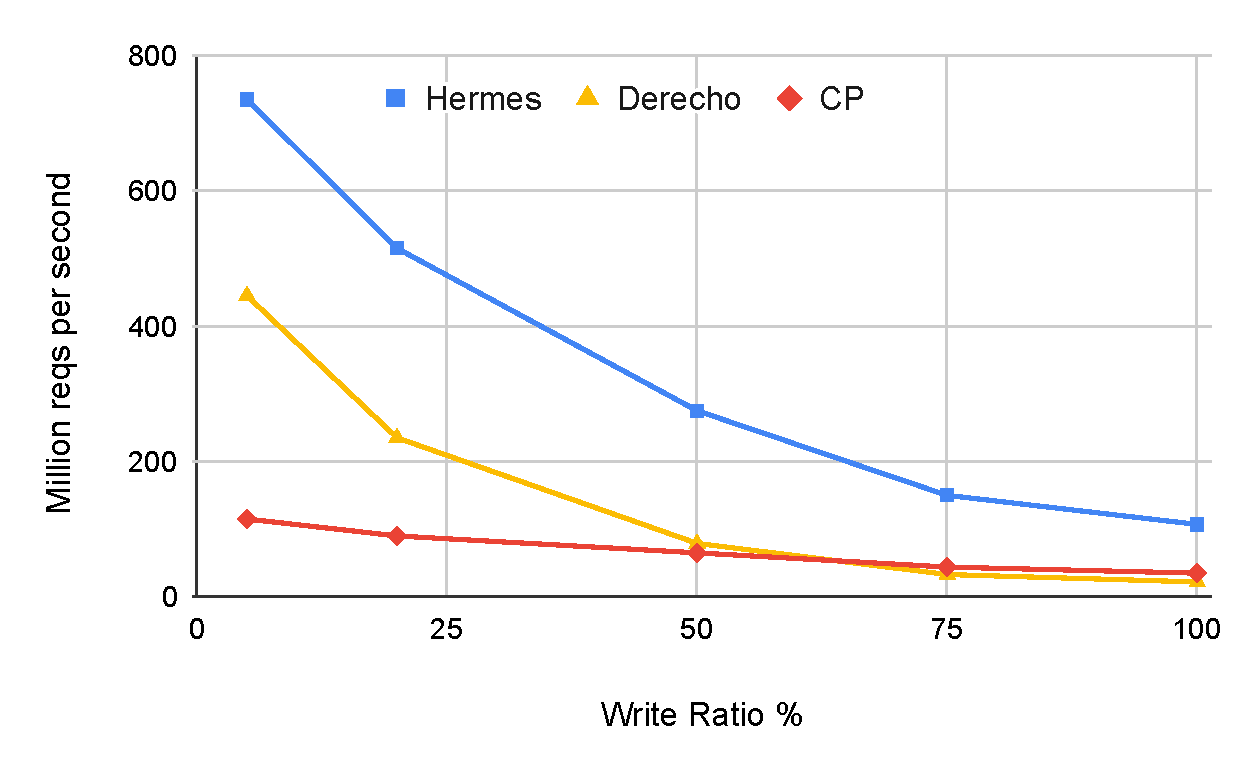
\includegraphics[width=\textwidth]{1_figures/hr-dr-cp.pdf}
    \captionsetup{width=\linewidth}
    % \vspace{-1.8em}
   \caption{Hermes, Derecho \& CP}
%   \vspace{-1.5em}
  \label{fig:hr-dr-cp}
  \end{subfigure}
  %
  \begin{subfigure}[t]{0.33\textwidth}
    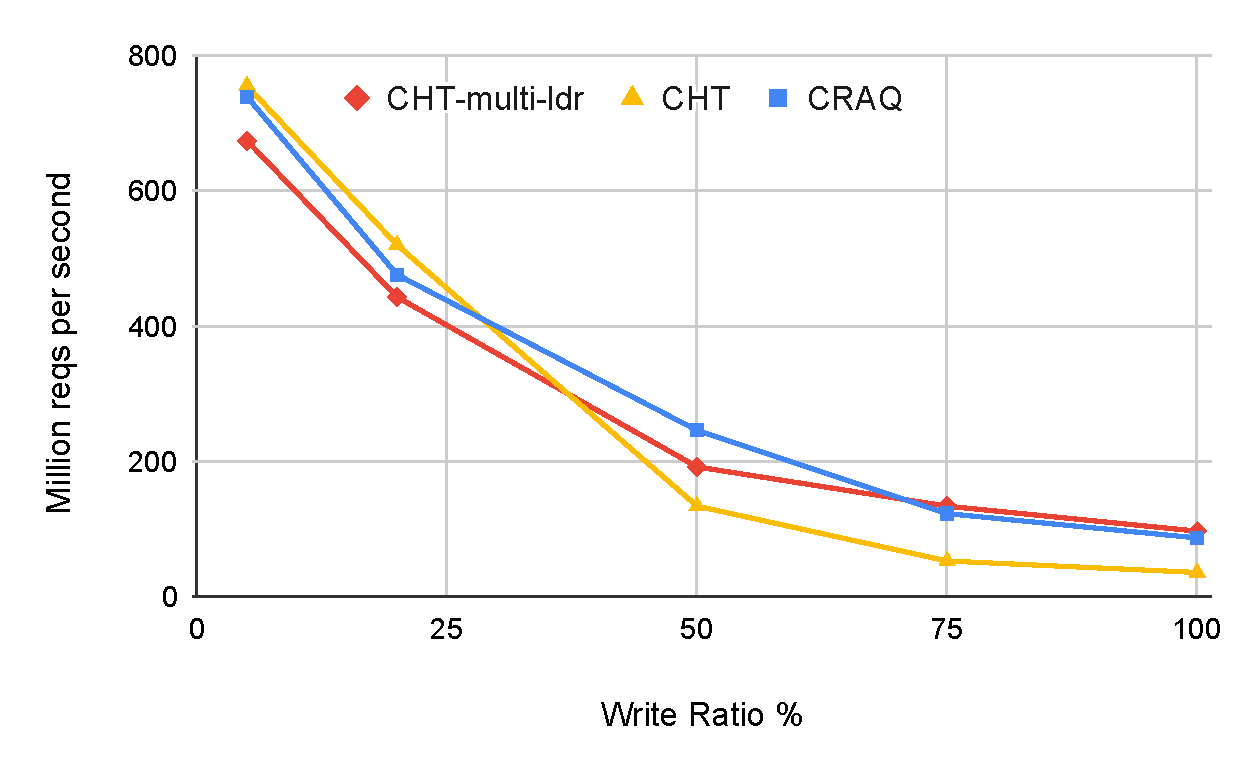
\includegraphics[width=\textwidth]{1_figures/craq-cht-chtml.pdf}
    \captionsetup{width=0.95\linewidth}
    % \vspace{-1.8em}
    \caption{CHT-multi-ldr, CHT \& CRAQ}
%   \vspace{-1.5em}
  \label{fig:cht-cht-craq}
  \end{subfigure}
  %
  \begin{subfigure}[t]{0.33\textwidth} 
  
    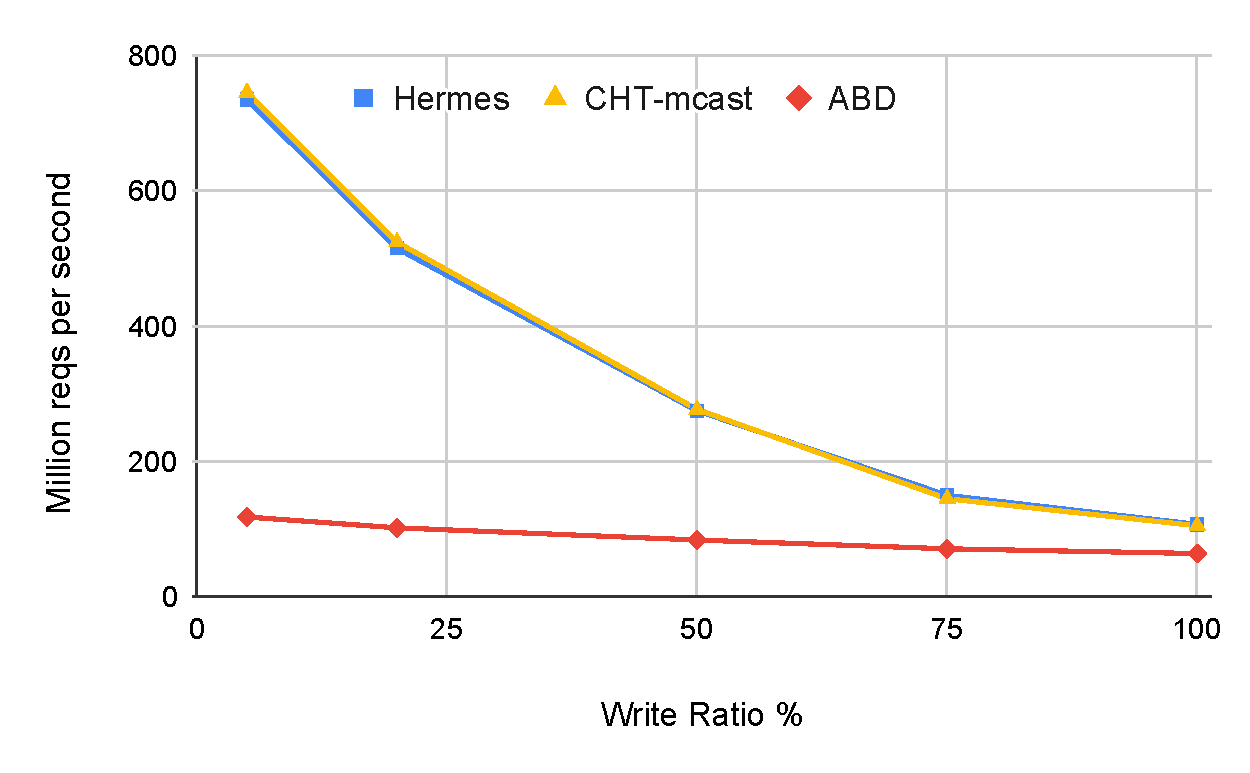
\includegraphics[width=\textwidth]{1_figures/hr-chtm-abd.pdf}
    \captionsetup{width=0.90\linewidth}
    % \vspace{-1.8em}
    \caption{Hermes, CHT-mcast \& ABD}
%   \vspace{-1.5em}
  \label{fig:hr-cht-abd}
  \end{subfigure}
%   \vspace{-1em}
  \caption{Throughput vs. write ratio}
  \label{fig:three-graphs}
%   \vspace{-1em}
\end{figure*}

% \begin{figure}[t]
%   \centering
%   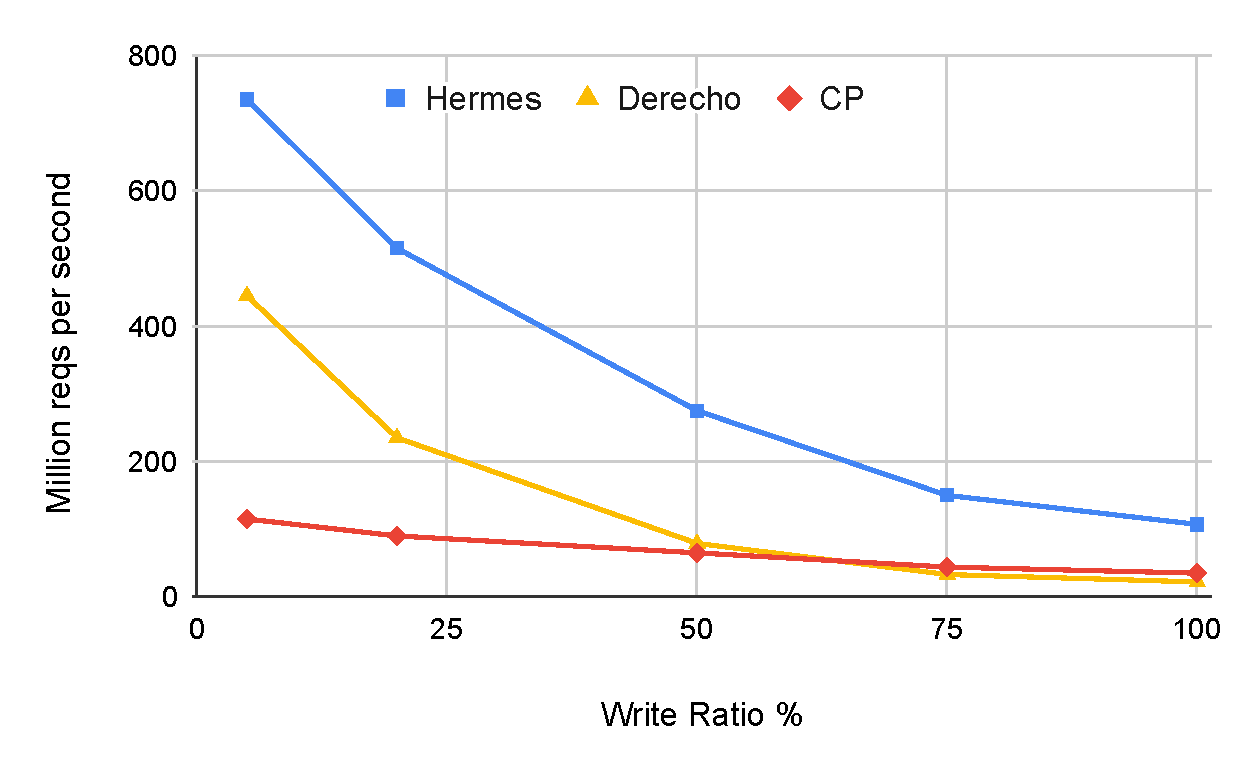
\includegraphics[scale=0.4]{1_figures/hr-dr-cp.pdf}
% %   \vspace{-0.5em}
%   \caption{Throughput of Hermes, Derecho \& CP, varying the write ratio from 1\% to 100\%}
% %   \vspace{-1.5em}
%   \label{fig:hr-dr-cp}
% \end{figure}

\subsection{\LPKO: CHT, CHT-multi-ldr, and CRAQ}\label{sec:ev:lpko}

We start the discussion of the \LPKO~protocols with CHT and then extend it to CRAQ. 


\beginbsec{CHT operation}
All writes in CHT are propagated to the leader. The leader completes the writes in two broadcast rounds, similarly to ZAB and MP, with two differences: 1) it does not create a total order of all writes and 2) it waits until a write has reached all followers before committing it. 
The latter allows for local reads at the follower nodes. Notably, reads need to block if there is an ongoing write to the same key, until that write commits. %



In CHT-multi-ldr each node is the leader for $1/N$ of all keys, with $N$ being the number of nodes. 
Upon receiving a write request for key $K$, the worker finds out the leader for that key through a simple modulo operation on the key. Then, similarly to CHT, the write is propagated to its leader, which executes it to completion. %


\beginbsec{CRAQ operation}
CRAQ organizes the nodes in a chain. All writes are steered to the head of the node, which then propagates them down the chain. When a write reaches the tail (\ie the last node of the chain), it is said to be committed and an ack propagates back, all the way to the head. On receiving the ack, nodes commit the write.
Reads are executed locally. As an optimization, reads do not block when there is an ongoing write to the same key, but instead are propagated to the tail. The tail is guaranteed to always know the latest committed write, because of its position in the chain. 



\beginbsec{Performance}
Firstly, recall that from \figref{fig:write-all}, we observed that CHT cannot balance the load and is bottlenecked by the send side of the leader, which saturates its NIC. There are three possible optimizations: using multiple leaders (CHT-multi-ldr), using a chain (CRAQ), and finally using the hardware multicast primitive (CTH-mcast). 

Notably, CRAQ has the lowest impact among the three techniques,
because it does not completely balance the load, as the tail does not contribute in the propagation of a write. In our 5-node deployment, the load is split between 4 nodes which explains why CRAQ reaches only 4/5 of the throughput of a well-balanced protocol such as CHT-mcast.

CHT-multi-ldr also falls short of CHT-mcast. The reason is a bit subtler. There is less opportunity to amortize cpu and network costs in CHT-multi-ldr, because writes need to be steered to different leaders. 
For example, assume that in our 5-node deployment a worker in one of the nodes receives 5 write requests from a client. Also assume that each request must be steered to a different leader. The worker cannot batch all messages to the same packet. Instead, it must create a packet for each of the writes, sending them to the different leaders. Furthermore the worker itself may be the leader for one of the writes, which means it must broadcast it, again losing the opportunity to batch it with other writes. 
Conversely, in vanilla CHT, the worker would simply batch all writes to the leader.

CHT-mcast enhances CHT with the multicast primitive.
In CHT, the send side of the leader is overloaded, because the leader broadcasts all writes, and every broadcast requires N unicasts (for N followers). However, the followers receive only one message from each broadcast, and thus when the leader utilizes $100$\% of its send bandwidth, the followers only utilize  $100/N$\% of their receive bandwidth.

CHT-mcast improves upon CHT exactly because in CHT the followers underutilize their receive side.
When the multicast primitive is used, the leader sends one message per broadcast instead of N. The preexisting underutilization in the followers' side allows us to leverage the leeway created by the multicast at the leader's send side, to send more writes to the followers.
Had there been no room in the receive side of the followers, the multicast would simply reduce the bandwidth used at the leader send side, without improving performance.
In fact this is exactly what happens for most of the broadcasting protocols (ABD, Hermes, CHT-multi-ldr, Derecho).
Notably, ZAB and MP, even though leader-based, are not scalable enough to tap into the multicasts benefits. %




\figref{fig:cht-cht-craq} shows the throughput of CHT-multi-ldr, CHT and CRAQ when varying the write ratio. Firstly note that CHT outperforms the other two for low write ratios.
This is because 1) CHT has a smaller work-per-request ratio and 2)~CHT is not bottlenecked by the leader's send side at low write ratios.
CHT's work-per-request ratio is smaller than CRAQs, because broadcasting writes is more efficient than propagating them through a chain, as it allows for a better amortization of compute and network costs.
CHT-multi-ldr has an even higher work-per-request ratio than CRAQ, because 
as the write ratio decreases, the opportunity to amortize costs by batching writes reduces, exacerbating its pre-existing problem. %
This is why it is outperformed by both CRAQ and CHT.
CHT-mcast scales CHT's throughput at high write ratios as it avoids the bottleneck in the leader's send side bandwidth.
As a result, its throughput is at the highest level for all write ratios, matching that of Hermes (\figref{fig:hr-cht-abd}).





\subsection{\DPKO: CP, All-aboard, ABD, and Hermes}\label{sec:ev:dpko}

Firstly we briefly explain the operation of the protocols and then discuss their performance.

 
\beginbsec{Operation}
In \DPKO~protocols, each node coordinates its own writes.
An ABD write requires two broadcast rounds. The first round finds out the version of the key stored in a majority of nodes and the second sends out the new value.
An ABD read requires one broadcast round with an optional second. The first round finds out the latest value from a majority of nodes. If the reader cannot infer from the replies to its first round that a majority of nodes store this value, then it performs a second round to broadcast it. Notably, the second round is not necessary in more than 99\% of the reads.

CP requires three broadcast rounds to complete a write: propose, accept and commit.
All-aboard is an optimization over CP, allowing a write to commit after two rounds when there are no conflicts or slow nodes, using CP as a fallback.
Both CP and All-aboard execute reads using ABD reads.
Finally, Hermes requires two broadcast rounds to complete a write. Its rounds are substantially more light-weight than CP and All-aboard (and even ABD) but all messages must always reach all nodes. For that reason, Hermes reads are local.



\begin{figure}[t]
  \centering
  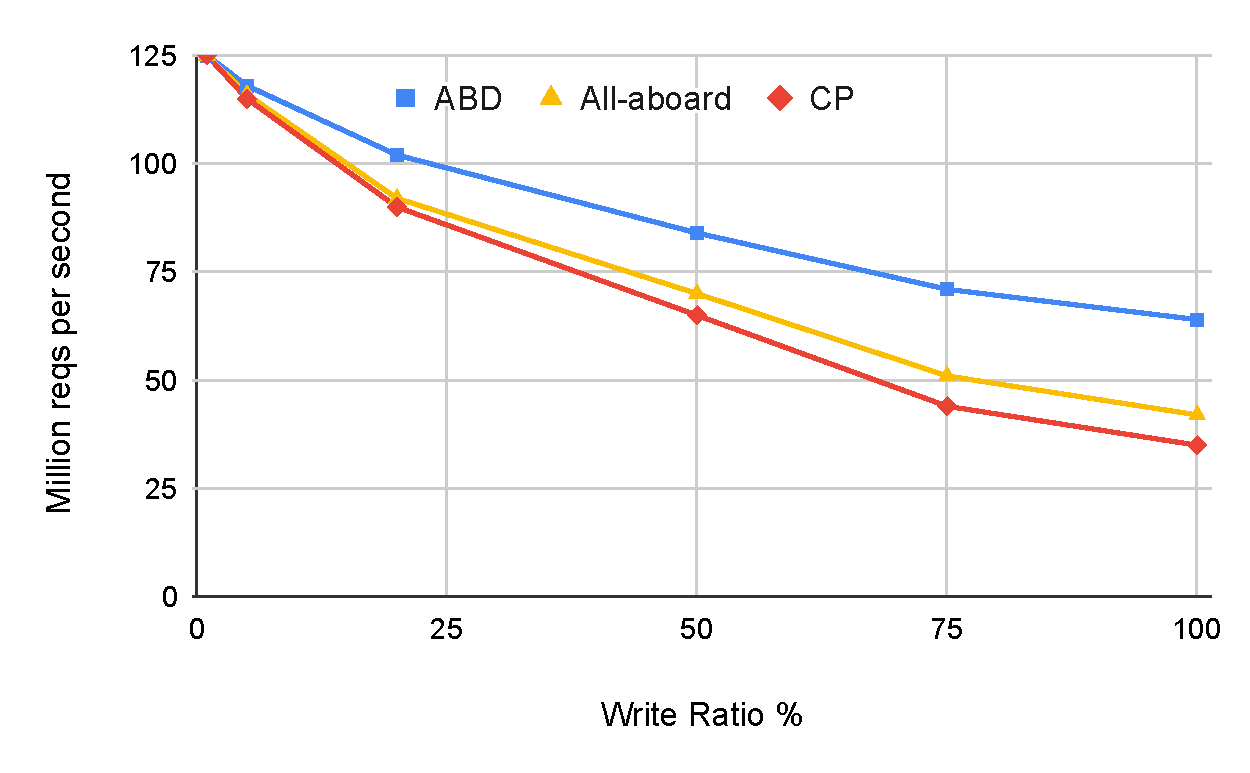
\includegraphics[width=0.4\textwidth]{1_figures/abd-ab-cp.pdf}
%   \vspace{-1.5em}
  \caption{Throughput vs write ratio for ABD, All-aboard \& CP}
%   \vspace{-1.5em}
  \label{fig:abd-ab-cp}
\end{figure}

\beginbsec{Performance}
Firstly, from \figref{fig:single-thr}, we observe that CP has the lowest single-threaded performance. This is because of the extremely high work-per-request ratio required in CP, as explained in \secref{sec:tax:dpko}. However,  CP is thread-scalable and well load balanced, enjoying a 10x improvement when multi-threaded (\figref{fig:write-all}) outperforming ZAB, MP and Derecho and matching CHT.

The All-aboard optimization reduces CP's high work-per-request but not completely.
This is why All-aboard is the second worse protocol when single-threaded.
Note that All-aboard has a significantly higher work-per-request ratio than Hermes and ABD, which also require two broadcast rounds. 
This highlights the fact that simply using the number of broadcast rounds as a metric to gauge performance is not sufficient. We need to factor in the size of the messages and the responses along with the complexity to create them.


Similarly to CP, All-aboard scales very well (10x) when multi-threaded, outperforming CP, CHT and the total order protocols.
Recall from \secref{sec:fail} that CP and All-aboard are the only two protocols (out of the \pnum) that can perform conditional writes while remaining available in the event of a failure. Therefore, for those keen on offering high availability, All-aboard comprises a great candidate, as it can also provide reasonably high performance.


ABD also offers the same levels of availability, but it is the only protocol out of the \pnum~that cannot perform conditional writes.
This simplification affords ABD a significantly lower work-per-request ratio than CP and All-aboard, which is why ABD outperforms CP and All-aboard both single-threaded and multi-threaded.
\figref{fig:abd-ab-cp} compares ABD, CP and All-aboard, varying the write ratio. Notably the read throughput is equal for all three, as they all implement ABD-reads. However, as the write ratio increases, ABD outperforms the other two due to its lower work-per-request ratio for writes.
Therefore, ABD comprises a great candidate, in cases where high availability is required and simple writes will suffice (as opposed to conditional writes).

\figref{fig:hr-cht-abd} compares ABD with Hermes (and CHT-mcast). Even though ABD is within a close distance in the write throughput, there is a big gap in the read throughput, demonstrating the cost of high availability. Specifically, Hermes mandates that every write reaches every node. In doing so, it concedes that all nodes must block on a failure (discussed in \secref{sec:fail}). However, it takes advantage of this concession in both reads and writes. In reads, by enabling them to execute locally, leveraging that all nodes have received the latest committed write. And in writes, by accelerating their operation, leveraging that a node that performs a write, has received all concurrent, conflicting writes.

This renders Hermes the better performing protocol out of all \pnum, making it an ideal candidate, for those who can afford an unavailability period in case of a failure.







